\chapter{Dynamic Programming}\label{chp:dynamic_programming}

% \lipsum[100]
% \blindtext[10]


The word \textbf{Dynamic} in Dynamic Programming refers that our computation complexity for the given problem can be reduced if:

\begin{enumerate}[(i)]
    \item Current state of the problem depends upon previous state solved.
    \item previous state has been already precomputed \& we have also saved their state.
\end{enumerate}


As we know recursion is way, in which current problem can be expressed in term of smaller sub-problem. Hence, writing the current state of problem in recursive way is the main step in solving question by dynamic programming.

\vspace{5mm}
% \addvspace{10cm}
Steps to Solve Dynamic Programming Question:
\begin{enumerate}[(i)]
    \itemsep0em 
    \item Express the current state of problem in recurrance relation.
    \item solve the problem in recursive way. (by considering all the edge case).
    \item Compute time complexity of recursive solution. Then compute time complexity of memoized solution.
    \item If memoized time complexiy is okay $\Rightarrow$ this is the solution.
    \item If memoized time compleixy is not okay $\Rightarrow$ express solution in alternative recurrance (same as modifying the recursive function defination) way; such that less variable term are mentioned in the recurrance relation.
\end{enumerate}

\section*{Dynamic Programming Questions}
\paragraph{type1} We will list \& discuss some of the common question pattern from this paradigm.

\part{Inclusion-Exclusion}
\begin{problem}{0/1 Knapsack}
    We are given N items where each item has some weight and profit associated with it. We are also given a bag with capacity W, [i.e., the bag can hold at most W weight in it]. The target is to put the items into the bag such that the sum of profits associated with them is the maximum possible. 
\end{problem}

\begin{solution}
    Try thinking in term of findAns(..) function.\\

    findAns(n,w,const arr) :: maximum profit associated when we have n items \& bag with capacity w.\\
   
    % //TO-DO: Make new environment to display them side by side
    Solution1:
    \begin{verbatim}
       int findAns(int n,int w,const vector<int>& arr)
       {
            if(w<=0) return INF; //invalid case, bag capacity must always be +v
            if(n<=0) return 0; //there is no item to chose from
           

            int inc = arr[n] + findAns(n-1,w-arr[w],arr);
            int exc =  findAns(n-1,w,arr);

            return max(inc,exc);
       }
    \end{verbatim}

way2: Process element from end.
    \begin{verbatim}
        int findAns(int idx, int w, const vector<int> &arr)
        {
            if(w <= 0) return INF;
            if(idx >= arr.size()) return 0;
            

            int inc = arr[idx] + findAns(idx+1,w-arr[idx],arr);
            int exc = findAnsans(idx+1,w-arr[idx],arr);
            
            return max(inc,exc);
        }
    \end{verbatim}

way3:(preferred) best for debugging \& visualization.

    \begin{verbatim}
        int findAns(int idx,int cw,const vector<int> &arr,const int W)
        {
            if(cw > W) return INVALID; //IMP: invalid case before valid case
            if(idx >= size) return 0;
           

            int inc = arr[idx] + findAns(idx+1,cw + arr[idx], arr,W);
            int exc = findAns(idx+1,cw,arr,W);

            printf("[%d,%d] : VAL(%d,%d)\n",idx,arr[idx],inc,exc);
            return max(inc,exc);
        }
    \end{verbatim}

Issue: you need to make sure inc does not get out of bound. You can do it in various way.


\begin{enumerate}[(i)]
    \item Instead of setting INVALID as INTMAX, set it as INTMAX/2.
    \item Instead of setting as extream large value. Set it to to some large value from question constrain. This way overflow can be avoided + you get your our INF for the given question.
\end{enumerate} 


way4:(preferred) Handling Invlaid cases during call itself (Hence, no need to handling invalid cases in base-case)

    \begin{verbatim}
        int findAns(int idx,int cw, const vector<int>& arr,int W)
        {
            if(idx >= 0) return 0;

            int inc = INVALID,exc = INVALID;

            if(cw + arr[idx] <= W)
                inc = arr[idx] + findAns(idx+1,cw+arr[idx],arr,W);
            
            exc = findAns(idx+1,cw,arr,W);

            printf("[%d,%d] : VAL(%d,%d)\n",idx,arr[idx],inc,exc);
            return max(inc,exc);
        }
    \end{verbatim}

    \paragraph{Summary Of Solutions:} All of the way written above shows same logic but implemented in different way.
    way3 and way4 produces good code which is easy to debug.
    Both is preferred way, if there are more decision making at current idx, then ideally way4 is preferred. (as you can see and modify all the decision at this step itself.)

\end{solution}
\begin{problem}{Coin Change}
    Given an integer array of coins[ ] of size N representing different types of currency and an integer sum, The task is to find the number of ways to make sum by using different combinations from coins[].
\end{problem}

\begin{solution}

    let f(idx,sum) :: number of ways to make sum with [0..idx] coin from the array.

    At index idx, we have two choice:
    (a) chose the current coin
    (b) do not chose the current coin
    
    \vspace{2mm}
    Recurrance Relation: $f(idx,sum) = f(idx,sum+arr[idx]) + f(idx+1,sum)$;

    Base Case: $idx >= 0 ,sum == SUM , sum > SUM$;

    \begin{verbatim}
        int findAns(int idx, int sum,const vector<int>& arr,const int SUM)
        {
            if(sum == SUM) return 1; //for current combination 1 SUM
            if(idx >= size) return 0; //no element => no way to make SUM
            if(sum > SUM) return 0;

            int inc = findAns(idx,sum+arr[idx],arr,SUM);
            int exc = findAns(idx+1,sum,arr,SUM);

            return inc + exc;
        }
    \end{verbatim}
  
\end{solution}
\begin{problem} {Rod-Cutting}
    Given a rod of length n inches and a
table of prices pi for i= 1,2,3...i determine the maximum revenue obtainable by cutting up the rod and selling the pieces. Note that if the price pn for a rod
of length n is large enough, an optimal solution may require no cutting at all.
\end{problem}

\marginnote{
    MarginNotes
}

\begin{solution}
    (1)
    \vspace{3mm}
    \hrule
    
    \begin{intution}
        Similarity to unbounded knapsack if we consider the solution array(sarr) derived from cost[].
    \end{intution}

        % 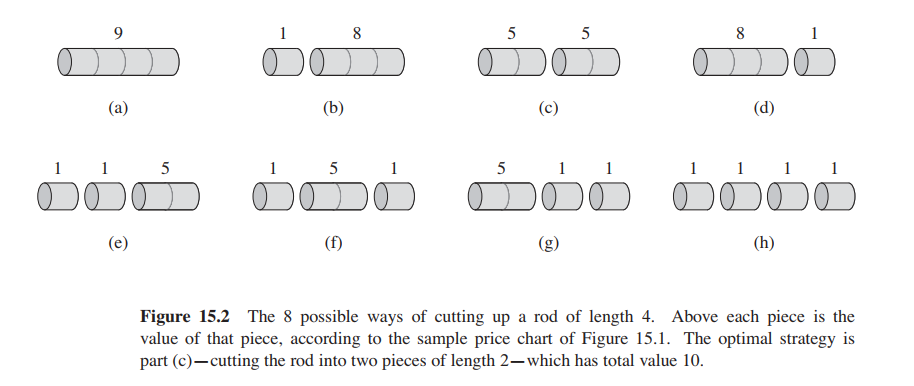
\includegraphics[width=10cm, height=5cm]{./diagram/rod-cutting-example.png}
        
       Considering the cost[], we will try to find sarr[]. \\
       where sarr[idx] := maximum revenue we can get if we are allowed to cut rod from length cost[0..idx-1]
       Now, for the sarr[] at index idx.
       We have two options:
        \begin{enumerate}[(a)]
            \item get the profit arr[idx] $\Rightarrow$ we can again cut the reduced rod with profit arr[idx] $val1 = cost[idx] + f(idx,n-(idx+1))$
            \item do not get the profit arr[idx] $val2 = f(idx+1,n)$
        \end{enumerate}
    \begin{verbatim}
        int findAns(int idx,int n ,const vector<int>& arr)
        {
            if(idx >= arr.size()) return 0;
            
            int val1 = INF; //inclusive : keep getting profit arr[idx] if its possible
            
            int val2 = INF; //exclusive: do not get profit arr[idx]
            
            int cut_length = idx+1;
            if(n-cut_length>=0)
                val1 = arr[idx] + findAns(idx,n-cut_length,arr); //rod-lenght is reduced
                
            val2 = findAns(idx+1,n,arr); 
            
            printf("[%d,%d]: (%d,%d)\n",idx,n,val1,val2);
            return max(val1,val2);
        }
    \end{verbatim}
\end{solution}


\begin{solution}
    (2)
    \vspace{3mm}
    \hrule
    
    \begin{intution}
        Consider the function signature as :
        $f(n) :=$ maximum revenu we can make if we have a rod of lenght n
    \end{intution}

    If we have rod of lenght n, that we can do cost.size() number of operations on this rod. (i.e we will try to cut this at all possible place)

    \begin{verbatim}
        int findAnsTwo(int n,const vector<int>& arr)
        {
            if(n<=0) return 0;
            int &mans = memt[n];
            if(mans != -1) return mans;

            int profit = INF;
            /* try to cut the rod in all possible way := cut the rod at 1,
            cut the rod at 2, ...
            */
            for(int k=1;k<=n;k++) //
            {
                int tprofit = arr[k-1] + findAnsTwo(n-k,arr); 
                /* question has 1 based index , so we do arr[k-1]*/
                profit = max(profit,tprofit);
            }

            return mans = profit;
        }
    \end{verbatim}
    
\end{solution}

% sol_file: /code/rod-cutting.cpp
\part{Ways at idx}
\begin{problem}{Matrix Chain Multiplication}
    Given a sequence of matrices, find the most efficient way to multiply these matrices together. The efficient way is the one that involves the least number of multiplications.
    The dimensions of the matrices are given in an array arr[] of size N (such that N = number of matrices + 1) where the ith matrix has the dimensions (arr[i-1] x arr[i]).
    \href{https://practice.geeksforgeeks.org/problems/matrix-chain-multiplication0303/1}{Pratice Link}
\end{problem}

\begin{solution}
    This is another important patter of dp. 
    In this, generally the size of array be such that we require $O(n^3)$ time complexiy to solve the question.
    
    % TO-DO: fix the marginote overflow issue
   \begin{marginnote}
    The $O(n^3)$ complexity of problem itself suggest that you should try this solution.
   \end{marginnote}

   \vspace{2mm}
   Here, instead of considering our question space to be [0..idx], we will consider it to be [l...r].


   And after that we will try to find our the number of ways can fill the carr[idx].

   \vspace{2mm}
   For the given problem, if we have the array at arr[l..r] and we need to find the optimal cost to multiply.
   Then we will try all possible way to multiply the matrix \& take the best amount them.
   
   \begin{verbatim}
        int matrixChainMultiplicatino(int l, int r, const vector<int>&arr)
        {
            if(l>=r)
                return 0; //no element exist in arrr

            int bCost = INT_MAX; //best cost
            
            //Try out all possible place
            for(int k=l;k<r;k++)
            {
                int leftCost =  matrixChainMultiplicatino(l,k,arr);
                int rightCost = matrixChainMultiplicatino(k+1,r,arr);

                cc printf("(%d,%d):: LeftCost = %d, RightCost = %d\n",l,r,leftCost,rightCost);

                int splittingCost = (arr[l-1] * arr[k] * arr[r]) + leftCost + rightCost;

                bCost = min(bCost,splittingCost);
            }
        //  printf("Best Cost to Multiply %d = %d\n",l,bCost);
            return bCost;
        }
   \end{verbatim}

\end{solution}

\begin{solution}
    //TO-DO: Complete this
    what if f(idx) := optimal multiplication cost when we have allowed only matrix arr[0...idx]

    for sarr[idx], the cost will depedent upon ??
\end{solution}
    

\part{Subsequence}
% Longest Common subsequeuen

\begin{problem}{Longest Common Subsequence(LCS)}
    Given two string s1 and s2. Find a new string which is the longest common substring of the given string.
    Practice: LC1143
\end{problem}

\begin{solution}[Inclusion-Exclusion]
    \obeylines
    In all string problem, we require to create some final string.
    In some of the problem, we are required to find the count (which is generally than 1e6).

    \medskip
    For all of problem in which we are asked max,min or count(below 1e6) we can try to construct the final string itself by following all the question constrain.

    \bigskip
    In current problem, let f(i,j,\_) := length of longest common subsequece when we are allowed to use s1[0..i] and s2[0...j] \textbf{only}.

    lets suppose we are also keeping track of lcs string formed up till now. let string formed till now as[0...idx].

    \medskip
    Now if know the subproblem, then at index idx - \textbf {we need to know as in how many ways we can fill the as[idx]}.

    \medskip
    Ways to fill:
    fill from s1, fill from s2. 
    two case: both same, both different.

   
    \begin{verbatim}
        \\Debug Version code
        int findAns(int i,int j,string as, const string &s1, const string &s2)
        {
            if(i>= s1.size() || j>= s2.size())  //if one is empty => we cannot find anything common now
                return 0; 
                
            //visualize the answer being created
            cc printf("\t:: [%s] (%s,%s)\n",as.c_str(),s1.substr(i).c_str(),s2.substr(j).c_str()); 
            
            int &mans = mem[i][j];
            int val1 = 0,val2=0,val3=0;
            
            if(s1[i] == s2[j])
            {
                val1 = 1 + findAns(i+1,j+1,as+s1[i],s1,s2);
            }
            else
            {
                val2 =  findAns(i+1,j,as+s1[i],s1,s2);
                val3 = findAns(i,j+1,as+s2[j],s1,s2);
            }
            
            //view all path computed at idx
            cc printf("[%s,%d,%d]: (%d,%d,%d)\n",as.c_str(),i,j,val1,val2,val3); 
            
            return mans = max({val1,val2,val3});
        }
    \end{verbatim}

\end{solution}

% TO-DO: add follow up environment here
% Follow-up Questions
Follow-Up Questions:
\begin{enumerate}[(a)]
    \item Find out the lcs string using mem matrix.
    \item  Find out the lcs string using dir matrix + iterative.
    \item Find out the lcs string using dir matrix + recursive.
\end{enumerate}

\begin{problem}{Edit Distance}
    You are given two string s1 and s2. Your task is to convert s1 to s2. But you have permitted following operations: Insert,Delete and Replace.

    \footnotetext{LC72}
\end{problem}

\begin{solution}[ways at idx]
    First try to formulate the question in term of recursive ways.

    We need to convert s1 to s2, but we have allowed only 3 operations.
    Hence, \intution{think of ways to fill the ansString, when we are at index idx.}

    \begin{code}
        int findAns(int i,int j,const string &s1,const string &s2)
        {
            cc printf("[%d,%d]\n",i,j);
            if(i==s1.size() && j==s2.size()) return 0;
            if(i>=s1.size()) return s2.size()-j; //add this much entry to s1
            if(j>=s2.size()) return s1.size()-i;  //delete this much entry from s1
            
            int &mans = mem[i][j];
            if(mans != -1) return mans;
            
            //now try to create new ansString.
            //to populate idx of answer string, you can have three operations
            
            int val1 = 1 + findAns(i,j+1,s1,s2); //insertion 
            int val2 = 1+ findAns(i+1,j,s1,s2); //deletion
            int val3 = 1 + findAns(i+1,j+1,s1,s2); //replacement
            int val4 = INT_MAX; //do nothing
            
            if(s1[i] == s2[j])
                val4 = findAns(i+1,j+1,s1,s2);
            
            return mans= min({val1,val2,val3,val4});
        }
    \end{code}
    
\end{solution}

\begin{pratice}
    \begin{asparaenum}
        \item Follow-Up: Can you devise the solution if the iCost,rCost and dCost values are not same?
    \end{asparaenum}
\end{pratice}
\begin{problem}{Longest Increasing Subsequnce}
    Given an integer array nums, return the length of the longest strictly increasing subsequence. LC 300\\
    (a)Give $O(n^2)$ algorithm.\\
    (b)Give $O(n*log(n))$ algorithm.
\end{problem}

\begin{solution}
    \vspace{2mm}
    \hrule
    \vspace{2mm}

    Standard recursive solution.
    let $f(idx,\_)$:= maximum lis length when we are allowed to chose element from [0...idx] \textbf{only}.

    \medskip
    Considerting we have answer for our subproblem.\\
    Then at index idx, we can fill up sarr[idx] in following ways:\\
    (a) pick arr[idx] if it satify the constrain\\
    (b) do not pick arr[idx]\\

    \begin{verbatim}
        int findAns(int idx,int last,vector<int> &sarr,const vector<int>&arr)
        {
            if(idx >= arr.size())
                return 0;
            
            /* for analysing the solution being created*\
    cc        printf("\t::[%d]: last(%d)\t",idx,last);
    cc        for(auto k:sarr) cout<<k<<" ";
    cc        cout<<endl;
                  
            int inc = 0; //Explain: why inc=1 is not the defult value?
            int exc = 0;
            
            if(last < arr[idx])
            {
                sarr.push_back(arr[idx]);
                inc = 1 + findAns(idx+1,arr[idx],sarr,arr);
                sarr.pop_back();
            }
            
            exc = findAns(idx+1,last,sarr,arr);   
            /* for analysing the optimal option to chose at index idx*/    
    cc      printf("[%d]:(%d,%d)\n",idx,inc,exc);
            
            return max(inc,exc);           
        }
    \end{verbatim}

    Follow-Up Question:\\
        (a) In case last in very big, how will you modify your solution so that its memoization is within time limit? (sol: see findAnsTwo)\\
        (b) Modify the solution of (a) and shift the invalid detection condition to recursion base condition. (sol: findAnsThree)

\end{solution}

\begin{solution}
    \obeylines
    \obeyspaces
    This is one of the DP approach where we will build the solution in iterative fashion.

    let dp[idx] := lenght of maximum lis \textbf{ending at idx.}
    \medskip
    Considering case when dp[0...idx-1] is know:
    Then for dp[idx], we can pair this up with all the dp[0...idx-1]. (with constrain satisfied)

    \begin{verbatim}
        int LISViaDP(vector<int>& arr)
        {
            int size = arr.size();
            
            vector<int> dp(size,1); //dp[idx] := lenght of longest lis which is ending at idx.
            
            for(int i=1;i<size;i++)
            {
                for(int j=0;j<i;j++)
                {
                    if(arr[i] > arr[j])
                        dp[i] = max(dp[i] , dp[j] + 1);
                }
            }
            
            int mx = 0;
            for(int i=0;i<dp.size();i++)
                mx = max(mx,dp[i]); 
            
            return mx;
        }
    \end{verbatim}
    

\end{solution}

\begin{solution}
    DP + Greedy\\
    Following up with the above solution.
    
    $dp[idx] = max(dp[idx] , 1+dp[j]) \forall \text{ j such that } arr[j] < arr[idx]$\\
    Can you the guess the subproblem dp[j] (for j<idx) which will give us the best result??

    \medskip
    Q: Out of various subproblem,can you chose specifc one \textbf{greedly}?? \newline

    \smallskip
    S: This is done by PatienceSorting algorithm first proposed by Hammersley.\\ In PatienceSorting, we maintain a seperate list of stack of cards.
        At each step we take an element from arr[] from left to right. Then try to place it on stack of cards availalbe.
        The stack is decreasing sequence.\\
        % TO-DO: add diagram: 
        
        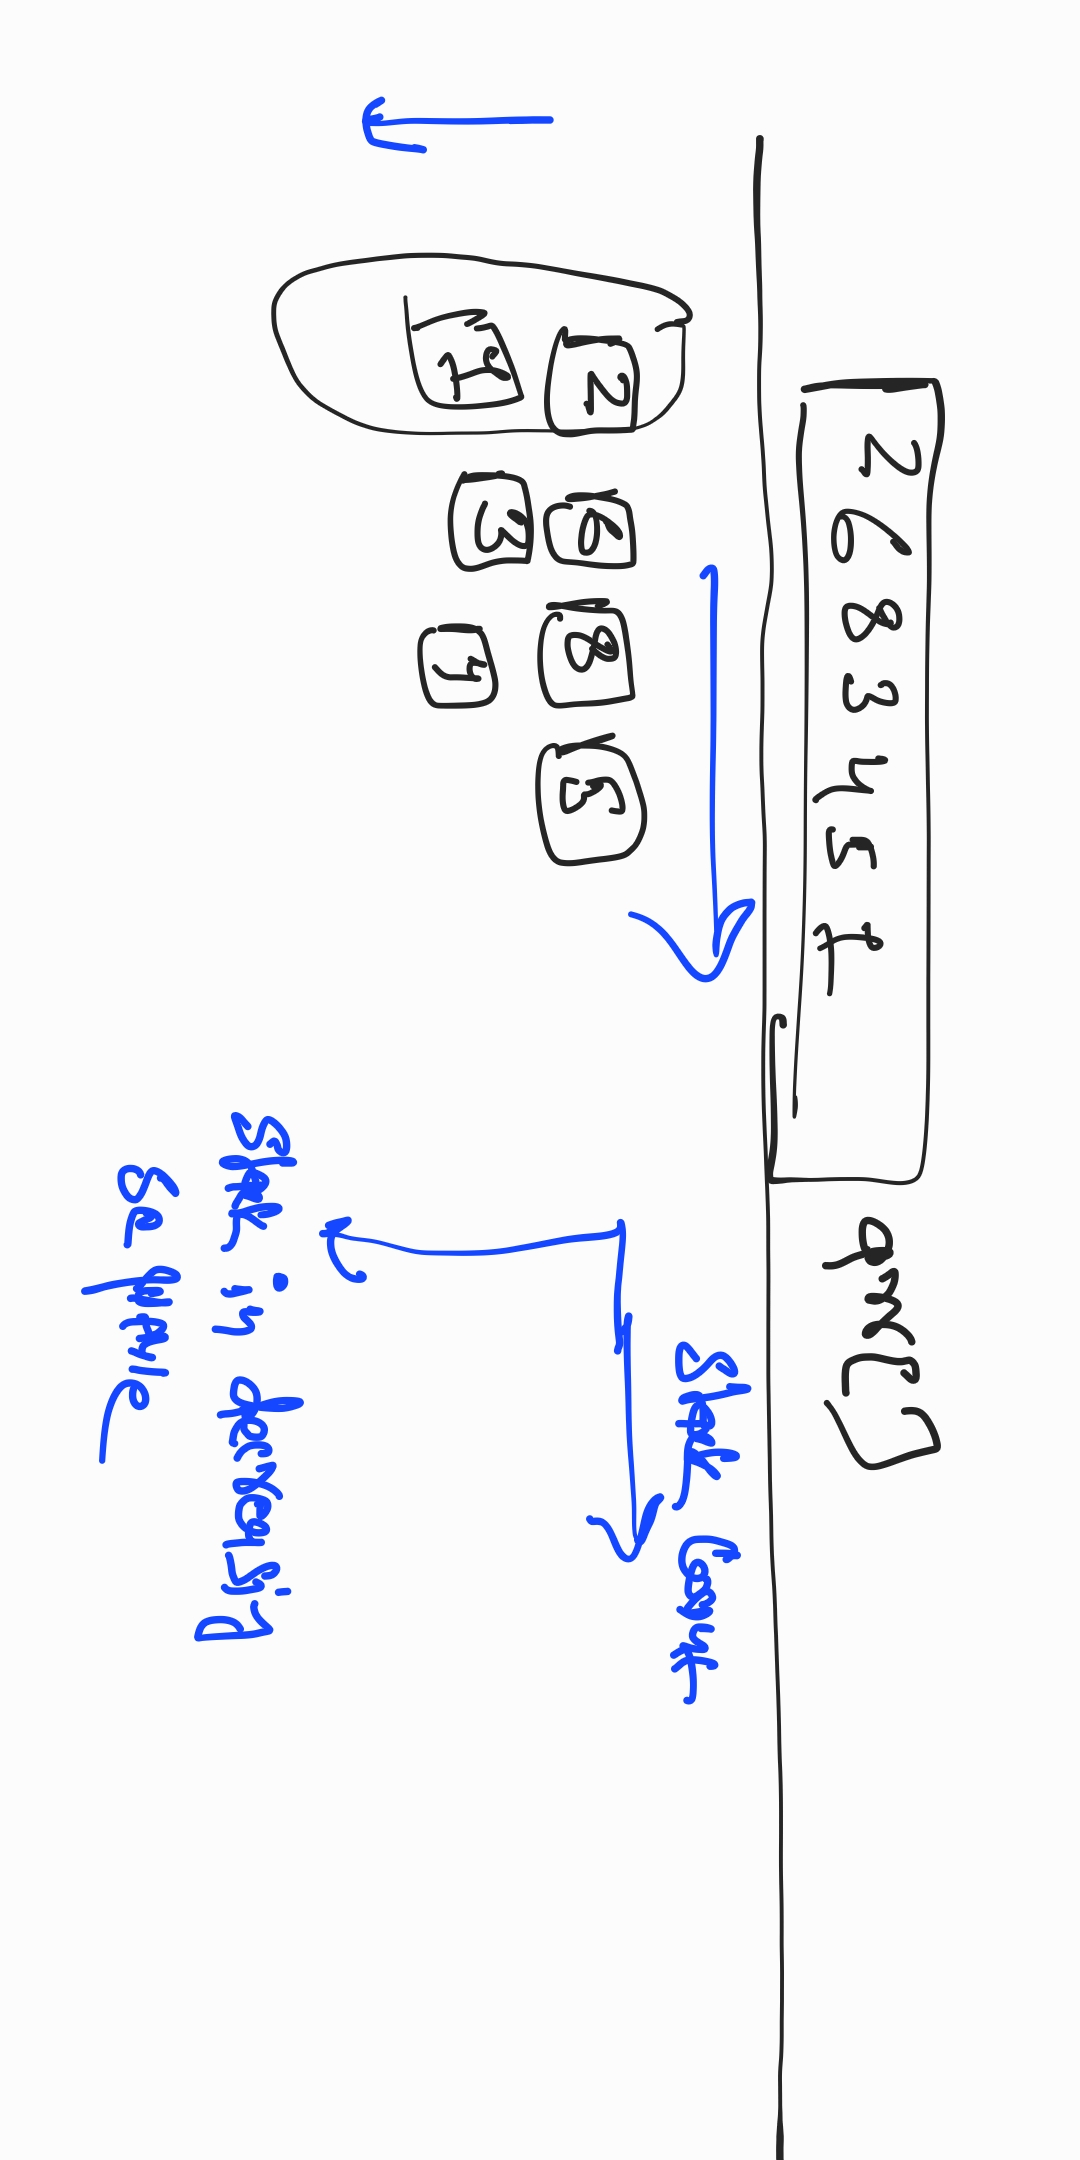
\includegraphics[angle=90,width=9cm,height=5cm]{./resources/PatienceSoring.jpg}
        
        (a) If this card is maximum amoung all the top cards of stack $\implies$ a new stack is created on right side.\\
        (b) If this card can be placed on top of some stack, then we chose the leftmost stack to place it upon.
        
        We keep repeating above operation keeping in mind that our goal is to minimize 

        See file /resource/LISPatienceSoring.pdf for more detail if you require.

    \begin{verbatim}
    int LICPatienceSorting(vector<int> &arr)
    {
        vector<int> sTop; 
        int size = arr.size();
        
        for(int i=0;i<size;i++)
        {
            int val = arr[i];
            
            //in all available stack, find the stack on which current element can be placed. 
            auto it = lower_bound(sTop.begin(),sTop.end(),val); 

            if(it == sTop.end())
            {
                /*current element is greator than all of the stack's top element => we need to 
                start a new stack*/
                sTop.push_back(val);
            }
            else
            {
                //we found a stack over which we can place the current element => place it on top
                int idx = it - sTop.begin();
            
                sTop[idx] = val; 
            }
        }//for loop ends here
        
        return sTop.size();
    }
    
    \end{verbatim}
\end{solution}

\begin{solution}
    There is one more interesting solution.
    The intution is that if we sort the array (lets call it sortedArr). And then if we find the Longest Common Subsequence
    between arr[] and sortedArray[] then it will be our LongestIncreasingSubsequence!!
\end{solution}

\begin{comment}
    % Below code is not so important, so skipped it
\begin{solution}
    Can you build up a recursive soltion with following defination:
    f(idx,\_):= maximum lis length ending at idx. \textbf{(i.e we must include idx)}

    considering that we know the subproblem answer.
    Then at index idx, we have following option:

    
    val1 = f(1) + 1 IF arr[1] < arr[idx]\\
    val2 = f(2) + 1 IF arr[2] < arr[idx]\\
    \dots\\
    $val_j = f(j) + 1 IF arr[j] < arr[idx] (for all j<idx)$

    we will take the best of all the options.

    Now, for f(idx) can you devise recursive relation?

    Code: see the findAnsFour(), some line in recursive solution is not so intutive.

    
\end{solution}
\end{comment}

% //To-DO Add pratice question environment.
Pratice Questions:
\begin{enumerate}[(i)]
    \item Follow-up question: for patience sorting algorithm. Can you print the LIS in O(n*long(n)) time?
    \item Can you print the patience soring stack, when the the array is [1,2,4,3,5,4,7,2]?
    \item LC2111  Minimum Operations to Make the Array K-Increasing.
    \item LC673  Number of Longest Increasing Subsequence. (First give a $O(n^2)$ solution, then improve it to O(log n)).
\end{enumerate}

\vspace{3cm}
Pratice Question Comment(Possibly hints too):
\begin{enumerate}[(i)]
    \item Follow the image for hint. 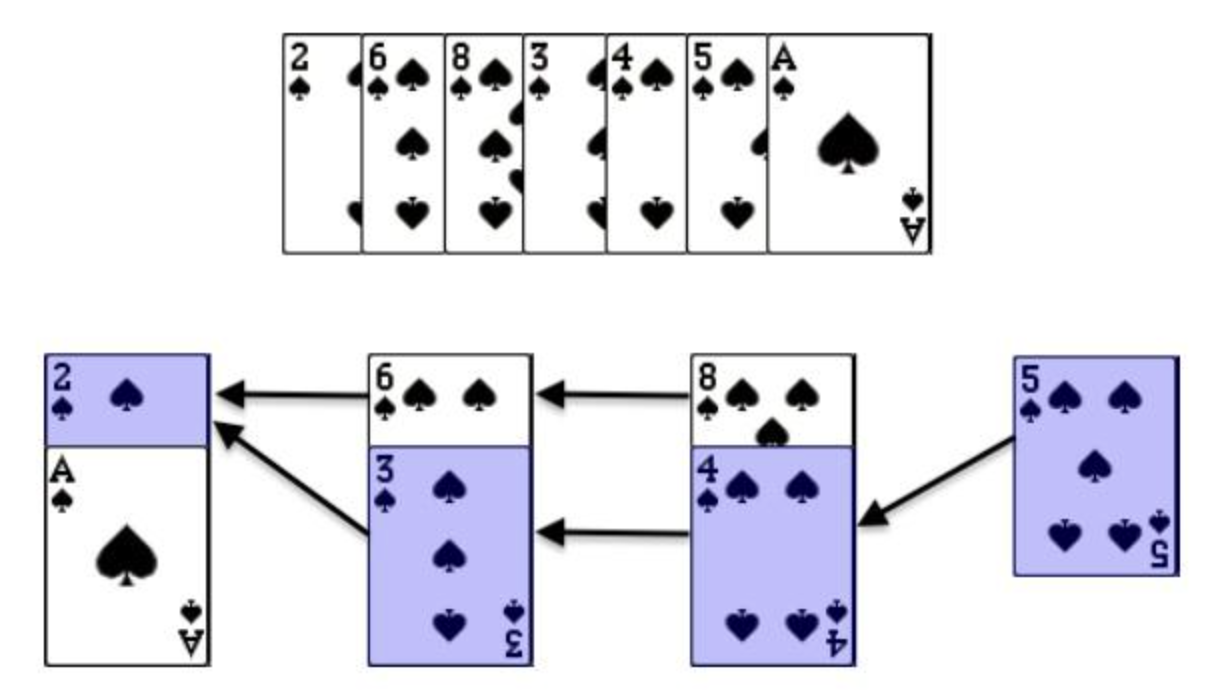
\includegraphics[width=5cm,height=3cm]{./resources/LICSequence.png}
    \item 
    \item LC2111 use $O(log(n))$ to determine LIS length. You can either use PatienceSorting to determine lis lenght in log(n) 
    \item we skipped O(long n) due to its solution complexity.(as at this level you also dont need it)
\end{enumerate}


\begin{problem}{Longest Palindromic Subsequence}
    Given a string s, find the longest palindromic subsequence's length in s.

    \footnotetext{LC516}
\end{problem}

\begin{solution}[Recursive]

    As the question ask us to find palindromic subsequence.  The palidromic pattern suggest us to find the recurrance relation involving start \& end of the current string.

    \intution{ let $f(l,r,\_)$ be the length of longest palindromic subsequence for string [l,r]}

    Now, there can be two case: either both are equal or they are not equal.

    \begin{code}
    int findLongestPalindrome(int l, int r, string s1)
    {
        if(l==r)
            return 1;
        if(l>r)
            return 0;
        
        if(s1[l] == s1[r])
            return 2+findLongestPalindrome(l+1,r-1,s1);
        else
        {
            int iLeft = findLongestPalindrome(l+1,r,s1);
            int iRight = findLongestPalindrome(l,r-1,s1);
            return max(iLeft,iRight);
        }
    }
    \end{code}
\end{solution}

\begin{solution}[Iterative]
    This can be achieved by transalation of above recursive.

    Alternative way of thinking the solution is, \rfl{try to build up the solution for lenght1, then lenght2 \dots lengthn}.

    i.e \intution{let dp[i][j] be the maximum lenght substring for string of s[i..j]. Assuming that you already know the answer of subsproblem. Can you express dp[i][j] in terms of lower lenght subsring?}

    \begin{marginfigure}
        
        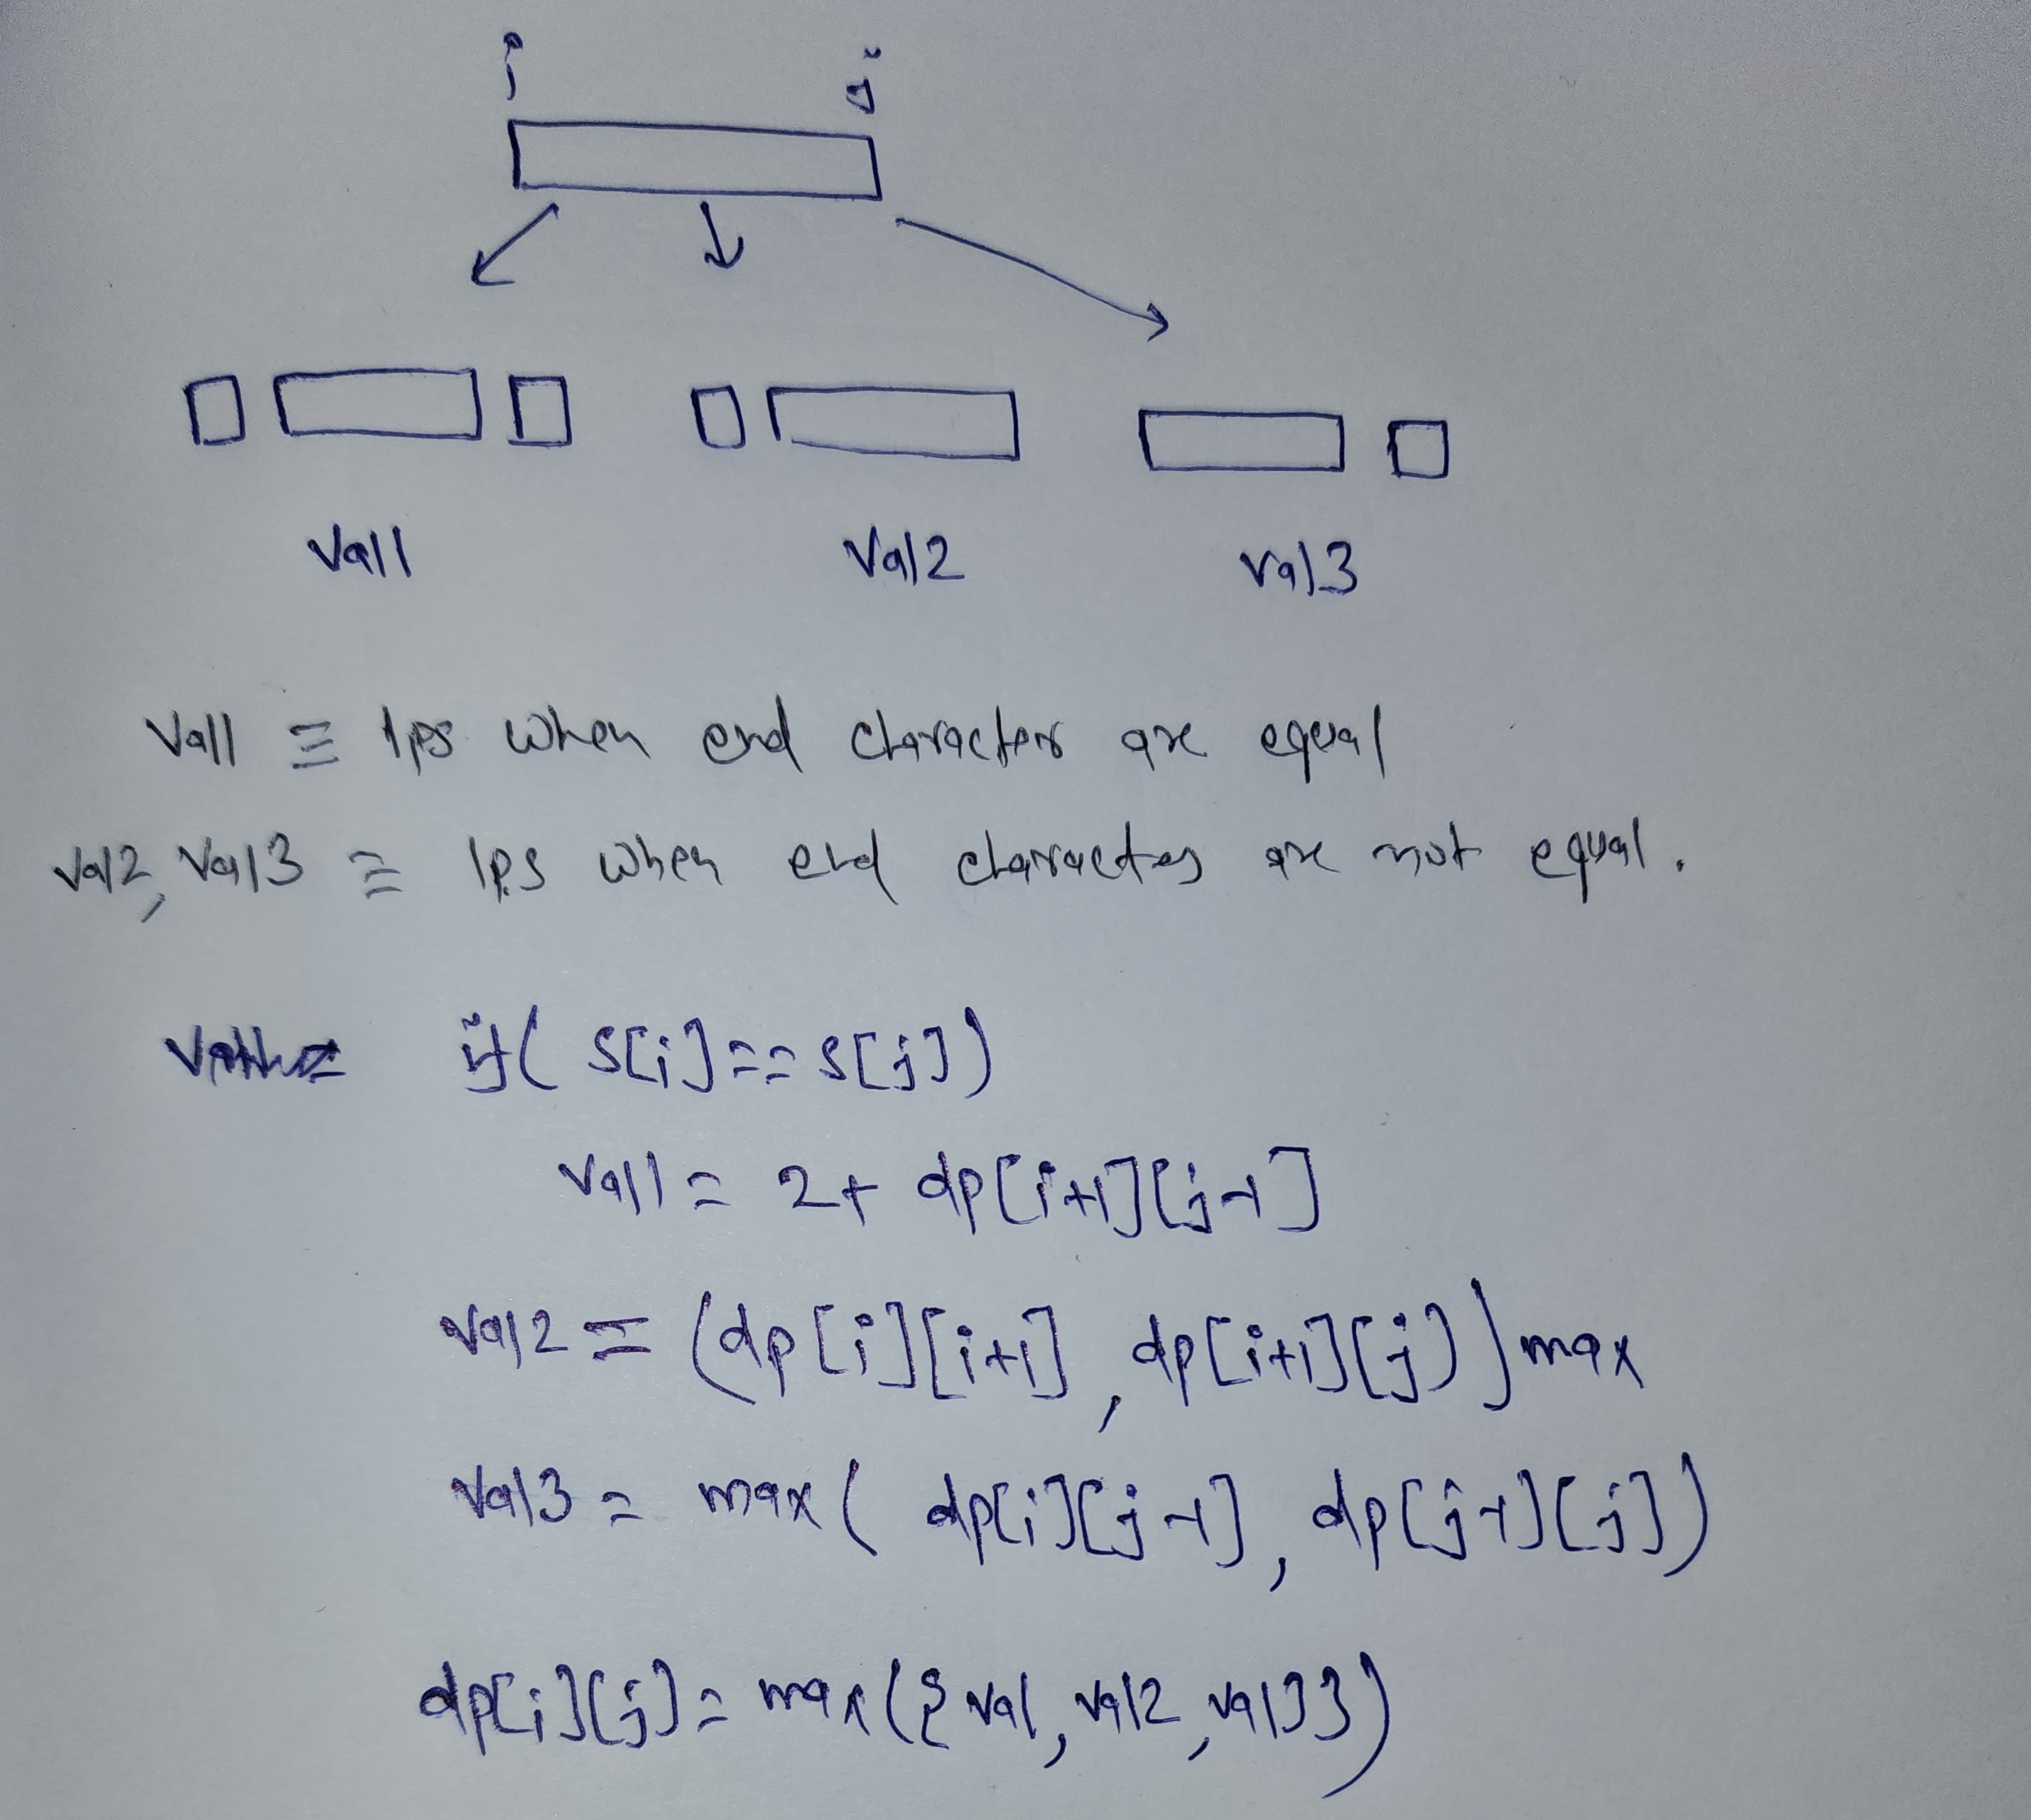
\includegraphics[width=\marginparwidth]{resources/LPS_Division1.jpg}  
    \end{marginfigure}

    \begin{figure}
        \centering
        \caption{Express dp[i][j] in subproblems}
        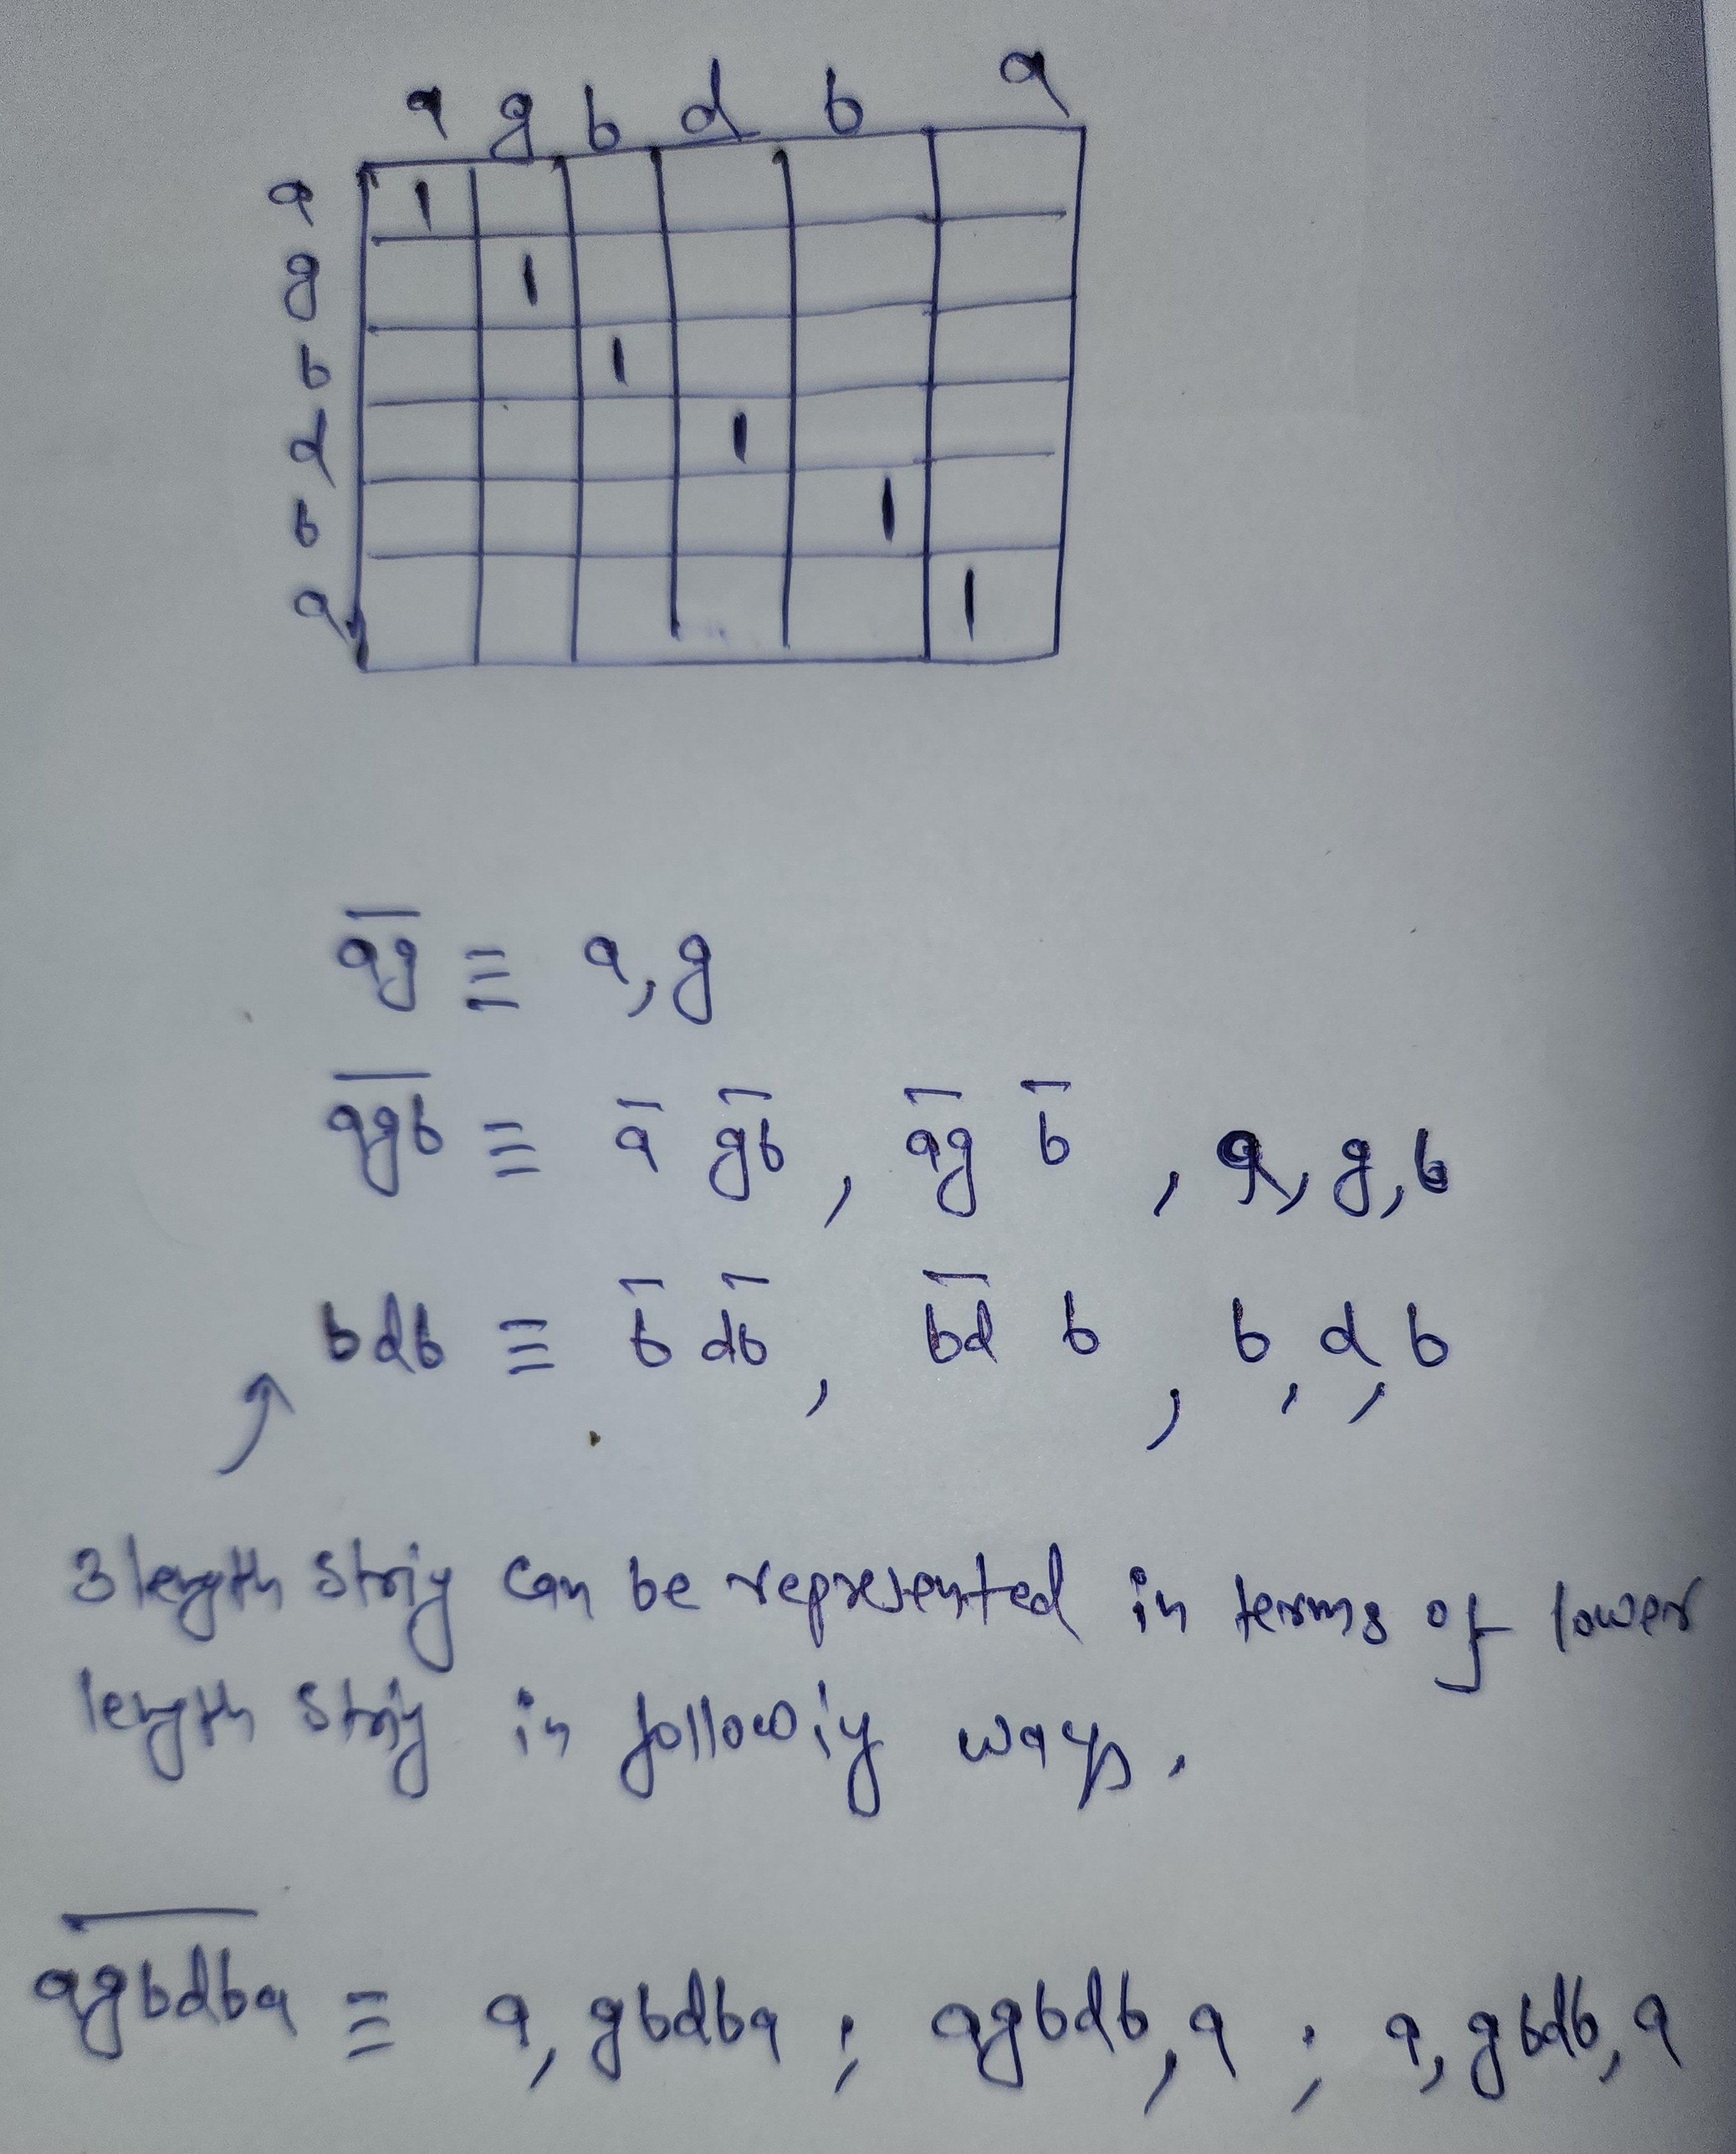
\includegraphics[width=\marginparwidth]{resources/LPS_Division2.jpg} 
    \end{figure}

    \begin{code}
        int longestPalindromeSubsequenceDP(string s1)
        {
            int NRow = s1.length();
            int NCol = s1.length();
        
            vector<vector<int> > dp(NRow,vector<int>(NCol,0));
        
            //Length 1 string is always valid palindrome withlength 1  
            for(int i=0;i<NRow;i++)
                dp[i][i] = 1;
        
            for(int l=2;l<=NRow;l++) //lenght = l
            {
                
                for(int i=0;i<NRow-l+1;i++) 
                {
                    int j = i+l-1; //r-l+1 = interval_size => j-i+1 = l => j = l+1-1
                        
                    int val=0;
                    if(s1[i] == s1[j]) //Recursion Translation
                    {
                        val = 2 + dp[i+1][j-1];
                    }
                    else
                    {
                        int iLeft = dp[i+1][j];
                        int iRight = dp[i][j-1];
                        val = max(iLeft,iRight);
                    }
                    dp[i][j] = val;
                }
            }      
            return dp[0][NCol-1];
        }
    \end{code}

 
    
\end{solution}

\part{Subarray Problem}

\begin{problem}{Longest Increasing Subarray | Kadan's Algorithm}
    You are given a array of number, find the longest \textbf{subarray} whose sum is maximum.
\end{problem}

\begin{solution}
    \rfl{For all subarray problem, please note that iterative solution is the most natural choise.}
    This is same as for all subsequence or subsequence count problem, recursion is the most natural choice.

    

    
\end{solution}
\begin{problem}{LC2771 Longest Non-decreasing Subarray From Two Arrays}
    You are give two array A and B of size n. $(n <= 10^5)$. Your task is to return the \textbf{maximum subarray length} in third array C. Where for c[i] in the range [0, n - 1], you can assign either A[i] or B[i].

    \footnotetext{Excellent Problem depicting key concept of recursion + past state in dp + subsequence vs subarray in recursion.}
\end{problem}

\begin{solution}[Recursion | Ways at idx(aka Inclusion-Exclusion)]

    Like all recursio problem subarray problem are not different.
    The only differance they posses from subsequence is that their element must be picked continously. We can include this informatin into pastState variable and code our solution.

    \medskip
    \intution{let $f(idx,pstate):=$ maximum subarray length if we are allowed to use arr[idx...size-1]  ONLY.}

    \medskip
    \rfl{Now as this is a state problem, each of the operation has a constrain applied to them.}

    \medskip
    For this problem, we have following options:
    \begin{enumerate}[(a)]
        \item \icode{int val1}: take from A. \\Restriction: can only be taken if its form a increasing subarray
        \item \icode{int val2}: take from B. \\Restriction: can only be taken if its form a increasing subarray
        \item \icode{int val3}: do not take.\\ 
        Restriction(subarray): for subarray problem, for this to happen we must have not picked any element previously.\\
        Restriction(subsequence):
        For subseqeunce problem, there will be no restriction on this.
    \end{enumerate}

    \begin{guide}
        Here is sample hint.

    \end{guide}
    % \newpage % pagebreak => spread text on previous page \newpage will not spread out the text

\begin{comment}
        Expeiremnt with \newpage if content is greator
    % \begin{mdframed}%[beforebreak=\newpage]
    \newpage
    \begin{code2}[Solution Captuion]

/* state=0 := no previous element was selected, state=1:= previous element was selected from A, state=:= previous element was selected from B*/
int findAnsFive(int idx,int pstate,vector<int>& A, vector<int>& B) /* pstate = previous state & NOT the current state, VERY important to make this observation*/
{
    if(idx >= A.size()) return 0;
    
    int &mans = mem[idx][pstate];
    if(mans != -1) return mans;
    
    /* at this time we have three options:
        (a) take from A
        (b) take from B
        (c) do not take (for subsequence this is always valid: but for subarray, this is only valid if we MUST HAVE  NOT PICKED any element previously)
    */
    /* Imp for subset sum, we was having two options: take from array , do not array*/
    
    int val1 = 0,val2=0,val3=0;
    
    int pelement = (pstate == 0) ? -1 :((pstate==1) ? A[idx-1]:B[idx-1]);
    
        if(pstate == 0) /* for subarray we can skip taking current element only if we have not taken any previous element*/
        val3 = findAnsFive(idx+1,0,A,B);
    
    if(pelement <= A[idx])
        val1 = 1 + findAnsFive(idx+1,1,A,B);
    if(pelement <= B[idx])
        val2 = 1 + findAnsFive(idx+1,2,A,B);
    
    
    
    return mans = max({val1,val2,val3});
}
\end{code2}

\begin{mdframed}[nobreak=true]
\begin{code2}[Hello Code]

    /* state=0 := no previous element was selected, state=1:= previous element was selected from A, state=:= previous element was selected from B*/
    int findAnsFive(int idx,int pstate,vector<int>& A, vector<int>& B) /* pstate = previous state & NOT the current state, VERY important to make this observation*/
    {
        if(idx >= A.size()) return 0;
        
        int &mans = mem[idx][pstate];
        if(mans != -1) return mans;
        
        }
\end{code2}
\end{mdframed}
        
\end{comment}

\begin{code3}[Code]
    /* state=0 := no previous element was selected, state=1:= previous element was selected from A, state=:= previous element was selected from B*/
    int findAnsFive(int idx,int pstate,vector<int>& A, vector<int>& B) /* pstate = previous state & NOT the current state, VERY important to make this observation*/
    {
        if(idx >= A.size()) return 0;
        
        int &mans = mem[idx][pstate];
        if(mans != -1) return mans;
        
        /* at this time we have three options:
            (a) take from A
            (b) take from B
            (c) do not take (for subsequence this is always valid: but for subarray, this is only valid if we MUST HAVE  NOT PICKED any element previously)
        */
        /* Imp for subset sum, we was having two options: take from array , do not array*/
        
        int val1 = 0,val2=0,val3=0;
        
        int pelement = (pstate == 0) ? -1 :((pstate==1) ? A[idx-1]:B[idx-1]);
        
            if(pstate == 0) /* for subarray we can skip taking current element only if we have not taken any previous element*/
            val3 = findAnsFive(idx+1,0,A,B);
        
        if(pelement <= A[idx])
            val1 = 1 + findAnsFive(idx+1,1,A,B);
        if(pelement <= B[idx])
            val2 = 1 + findAnsFive(idx+1,2,A,B);
        
        
        
        return mans = max({val1,val2,val3});
    }
    \end{code3}

\end{solution}

\begin{pratice}
    Follow-Up and  Pratice problems:
    \begin{asparaenum}[(a)]
        \item Follow Up 1: Can you modify the above algorithm so that f(idx,pstate) defination changes as. \icode{f(idx,pstate)=  Maximum lenght of subarray that start at idx. and} \rfl{must include idx}
        \item Can you implement the same code when we go from right to left in recurison. ie we start with \icode{f(n,pstate)} and its state depends upon n-1. (this is not much important, but just for case you should know that we can code this way also.)
        
        \item Can you devise iterative solution follwing the above code?
        \item Can you devise iterative solution following the follow-up-1 code.
        
        \item How will you modify the solution if there are k arrays to chose from?? What will the time comlexity?
        \item Explain how the solution changes if the question was about finding subsequence instead of subarray. Justify your logic and  code it.
        \item For subsequnce problem, justify why code complexity increases to $O(n*n)$ where for array it was just $O(n*3)$
        \item Their exist a patience sorting algorith for longest incerasing subsequence. which gives the lenght of lcs in $O(n*log(n))$ time. Which is better that our current $O(n^2)$ solution. Discuss how the question can be modified to force us use the patience sorting for lcs.
    \end{asparaenum}
\end{pratice}

\vspace{1cm}
\begin{pratice}
    Hints for follow up:
    \begin{asparaenum}[(a)]
        \item Follow Up 1: if you remove the variable \icode{val3},  then \icode{f(idx,pstate)} changes such that it contains the maxium lenght that MUST stat from idx. and MUST include idx. \rfl{to get the answer now, you will need to have gmx}
        \item See findAnsSix from file LC2771.cpp
        \item for follow-up-1 iterative see function findIterative in file LC2771.cpp
    \end{asparaenum}
\end{pratice}

\begin{pratice}
    Similary Problem list, that is bases on pstate. (can require subarray or subsequence):
    \begin{asparaenum}
        \item LC354 Russian Doll Envelopes
        \item LC646 Maximum Length of Pair Chain
        \item TO-DO: Add more item
    \end{asparaenum}
\end{pratice}
\begin{problem}{Longest Palindromic Subarray}
    Given a string s, find the lenght of longest palindromic subarray in s.

    \footnotetext{LC5}
    
\end{problem}

\begin{solution}

    \begin{guide}
        TO-DO: Remove parenthesis guides hints.
        
        \item First try with generating all substring. Can you do it in $O(n^2)$ ?

        \item
        If you define your problem statement with l..r range. You have the following defination \verb|f(l,r):= | length of longest valid palindromic substring when you are allowed to use \verb|arr[l..r]| \textbf{only}. \\
        The drawback of this is that it convert your complexity to $O(n^2)$

        \item
        \rfl{If you can define what will be the increment during inclusion of idx. Then you can use Inclusion-Exclusion pattern to solve this problem.}
        
        way1: \verb|f(idx,_):=| lenght of longest palindormic subarray when we are allowed to use $arr[0..idx]$ \textbf{only}.

        way2: \verb|f(idx,_):=| length of longest palindromic subarray ending at idx \textbf{that must include idx}. (OR startign at idx and must include idx). 

       \intution{As we know way1 is preferred with subsequence problem and way2 is preferred for subarray problem.}
       Lets try to solve current subarray via way2.

       \item Can you think of a solution using stack?
       
       \item Can you think of a solution that usages expand around center approach?
       
       \item Do you know about Manacher's Algorithm? Which solves this problem in linear time.
    


    \end{guide}
\end{solution}

\begin{pratice}

    \begin{enumerate}
        \item 
    \end{enumerate}

\end{pratice}

\begin{praticeHints}
    \item LC32 
\end{praticeHints}


\begin{exercise}
    \begin{enumerate}
    \item (LC 1547) Minimum cost to cut a stick.
    \item  For LC1547 print the optimal ordering.
    \item 
    LC 2218 : $f(idx,\_)$ = maximum total value of coing we can pick if we are allowed to pick coins from from arr[0...idx]\\
    now at idx, we have the option to chose either \begin{verbatim} {1}, {1,2}, {1,2,3}... {1,2,...min(k,size)} \end{verbatim} options
       
    we will take the best from all the option.
   
    \item LC 1105: with $f(idx,\_)$ defination as same as 2218.\\
    At idx, we can chose either 1 or 2 or 3 books, ... n books. We will take the best of all.

    \item LC 1547 (simple variation of rod-cutting)
    \item LC 1092- Shortest Common Supersequence
    \item LC801 Minimum Swaps To Make Sequences Increasing 
    \item LC139 Word Break\\ Given a string s and a dictionary of strings wordDict, return true if s can be segmented into a space-separated sequence of one or more dictionary words.
    \item SEPERATOR (Please Categorize)
    \item 
    LC 2218 : $f(idx,\_)$ = maximum total value of coing we can pick if we are allowed to pick coins from from arr[0...idx]\\
    now at idx, we have the option to chose either \begin{verbatim} {1}, {1,2}, {1,2,3}... {1,2,...min(k,size)} \end{verbatim} options
       
    we will take the best from all the option.
   
    \item LC 1105: with $f(idx,\_)$ defination as same as 2218.\\
    At idx, we can chose either 1 or 2 or 3 books, ... n books. We will take the best of all.

    \item LC 1547 (simple variation of rod-cutting)
    \item LC 1092- Shortest Common Supersequence
    \item LC801 Minimum Swaps To Make Sequences Increasing 
    \item LC139 Word Break\\ Given a string s and a dictionary of strings wordDict, return true if s can be segmented into a space-separated sequence of one or more dictionary words.
\end{enumerate}


    { \Large Palindrome Pattern \\}
    In this pattern, range is decided by arr[l..r]. Or arr[0..l] for some case.
    \begin{enumerate}
        \item (LC131) Palindrome Partioning \\Given a string s, partition s such that every substring of the partition is a palindrome. Return all possible palindrome partitioning of s. 
        \constrain{s.lenght<=16, s[i] \in [a,z]}
        
        \item (LC132) Palindrom Paritioning II \\ For above question, return minimum cuts needed to perform the operation.
        \constrain{s.lenght\leq2000,s\in[a-z]}

        \item (LC1216) Valid Palindrome \\A string is k-palindrome if it can be transformed into a palindrome by removing at most k characters from it. Given a string s and an integer k, return true if s is a k-palindrome.
        \constrain{s.lenght \leq 1000, k \leq s.length, s \in [a-z]}

        \item (LC1246) Palindrome Removal\\ You are given an integer array arr.
        In one move, you can select a palindromic subarray \verb|arr[i], arr[i + 1], ..., arr[j] where i <= j|, and remove that subarray from the given array.
        Return the minimum moves to remove all element from the array.
        \constrain{arr.length \leq 100, arr[i] \in [1,20]}

    \end{enumerate}

\end{exercise}

\begin{exerciseHints}[Solutions/Comments:]
    % Comment About Excercise Problem (And possibly have hint too)
    \begin{enumerate}
        \item LC801: Nice problem where state information can be transferred to other variable + if we use base case to detect invalid case, then code can be greatly simplified.
        \item LC139 Word Break \\Give (a) f(idx,\_) solution (b) f(l,r,\_) solution (c) BFS Solution (d) Trie Solution
    \end{enumerate}

    { \Large Palindrome Pattern(almost all dp pattern here) \\}
    \begin{enumerate}
        \item (LC131) Palindrome Partioning \\As the constrain is less, can you backtract all possible combination? Let \verb|f(idx):=| generate the answer when you are given \verb|arr[idx:]| only.
        
        \item (LC132) You can try brute forcing, but now as the constrain reqirement suggest us to use $O(n^2)$ algorithm.
        
        Let \verb|f(l,r):=| minimum cut needed to partion all substring as plaindrome, when you are allowed to use \verb|arr[l..r]| only. Then for each \verb|f(l,r)| you can try cutting at all places and take the best of cost.
        Explain why the complexity is $O(n^2)$ even though we haved used two variable l and r. And we are splittin at all k places also.
        
        If you think your recursive function defination as \verb|f(idx):=| minimum cut need when you are allowed to use \verb|arr[idx:]| only. Then at each idx, you can try to form a substring \verb|s[idx:k]|. If this substring is itself a plaindrome, the problem to \verb|f(k)|.

        There exist other approach, expand around the center. Can you write the code for all 3 above approaches?

        \item (LC1216) Valid Palindrome\\ Try to solve it just like you have solved Edit Distance. Start with l and r pointer, if both equal then no cost to delete. if equal then try deleting left, then right.
        take minimum cost from all three operation.

        LCS way:Alternative approach is to reverse the given string and find maximum subsequence length between the two. The string is k-palindromic if the difference between the string length and subsequence length is not more then k.
        
        \item (LC1246) Palindrome Removal \\Key Observation: A[i] can be deleted either alone or can make a pair. Now in normal \verb|palindrome length| calculation, we make A[l] pair with A[r] (A[r] is first occurrance from right side for arr[l..r]). But, in current case A[i] can me made to pair with all ch which occurr at any index.
        
        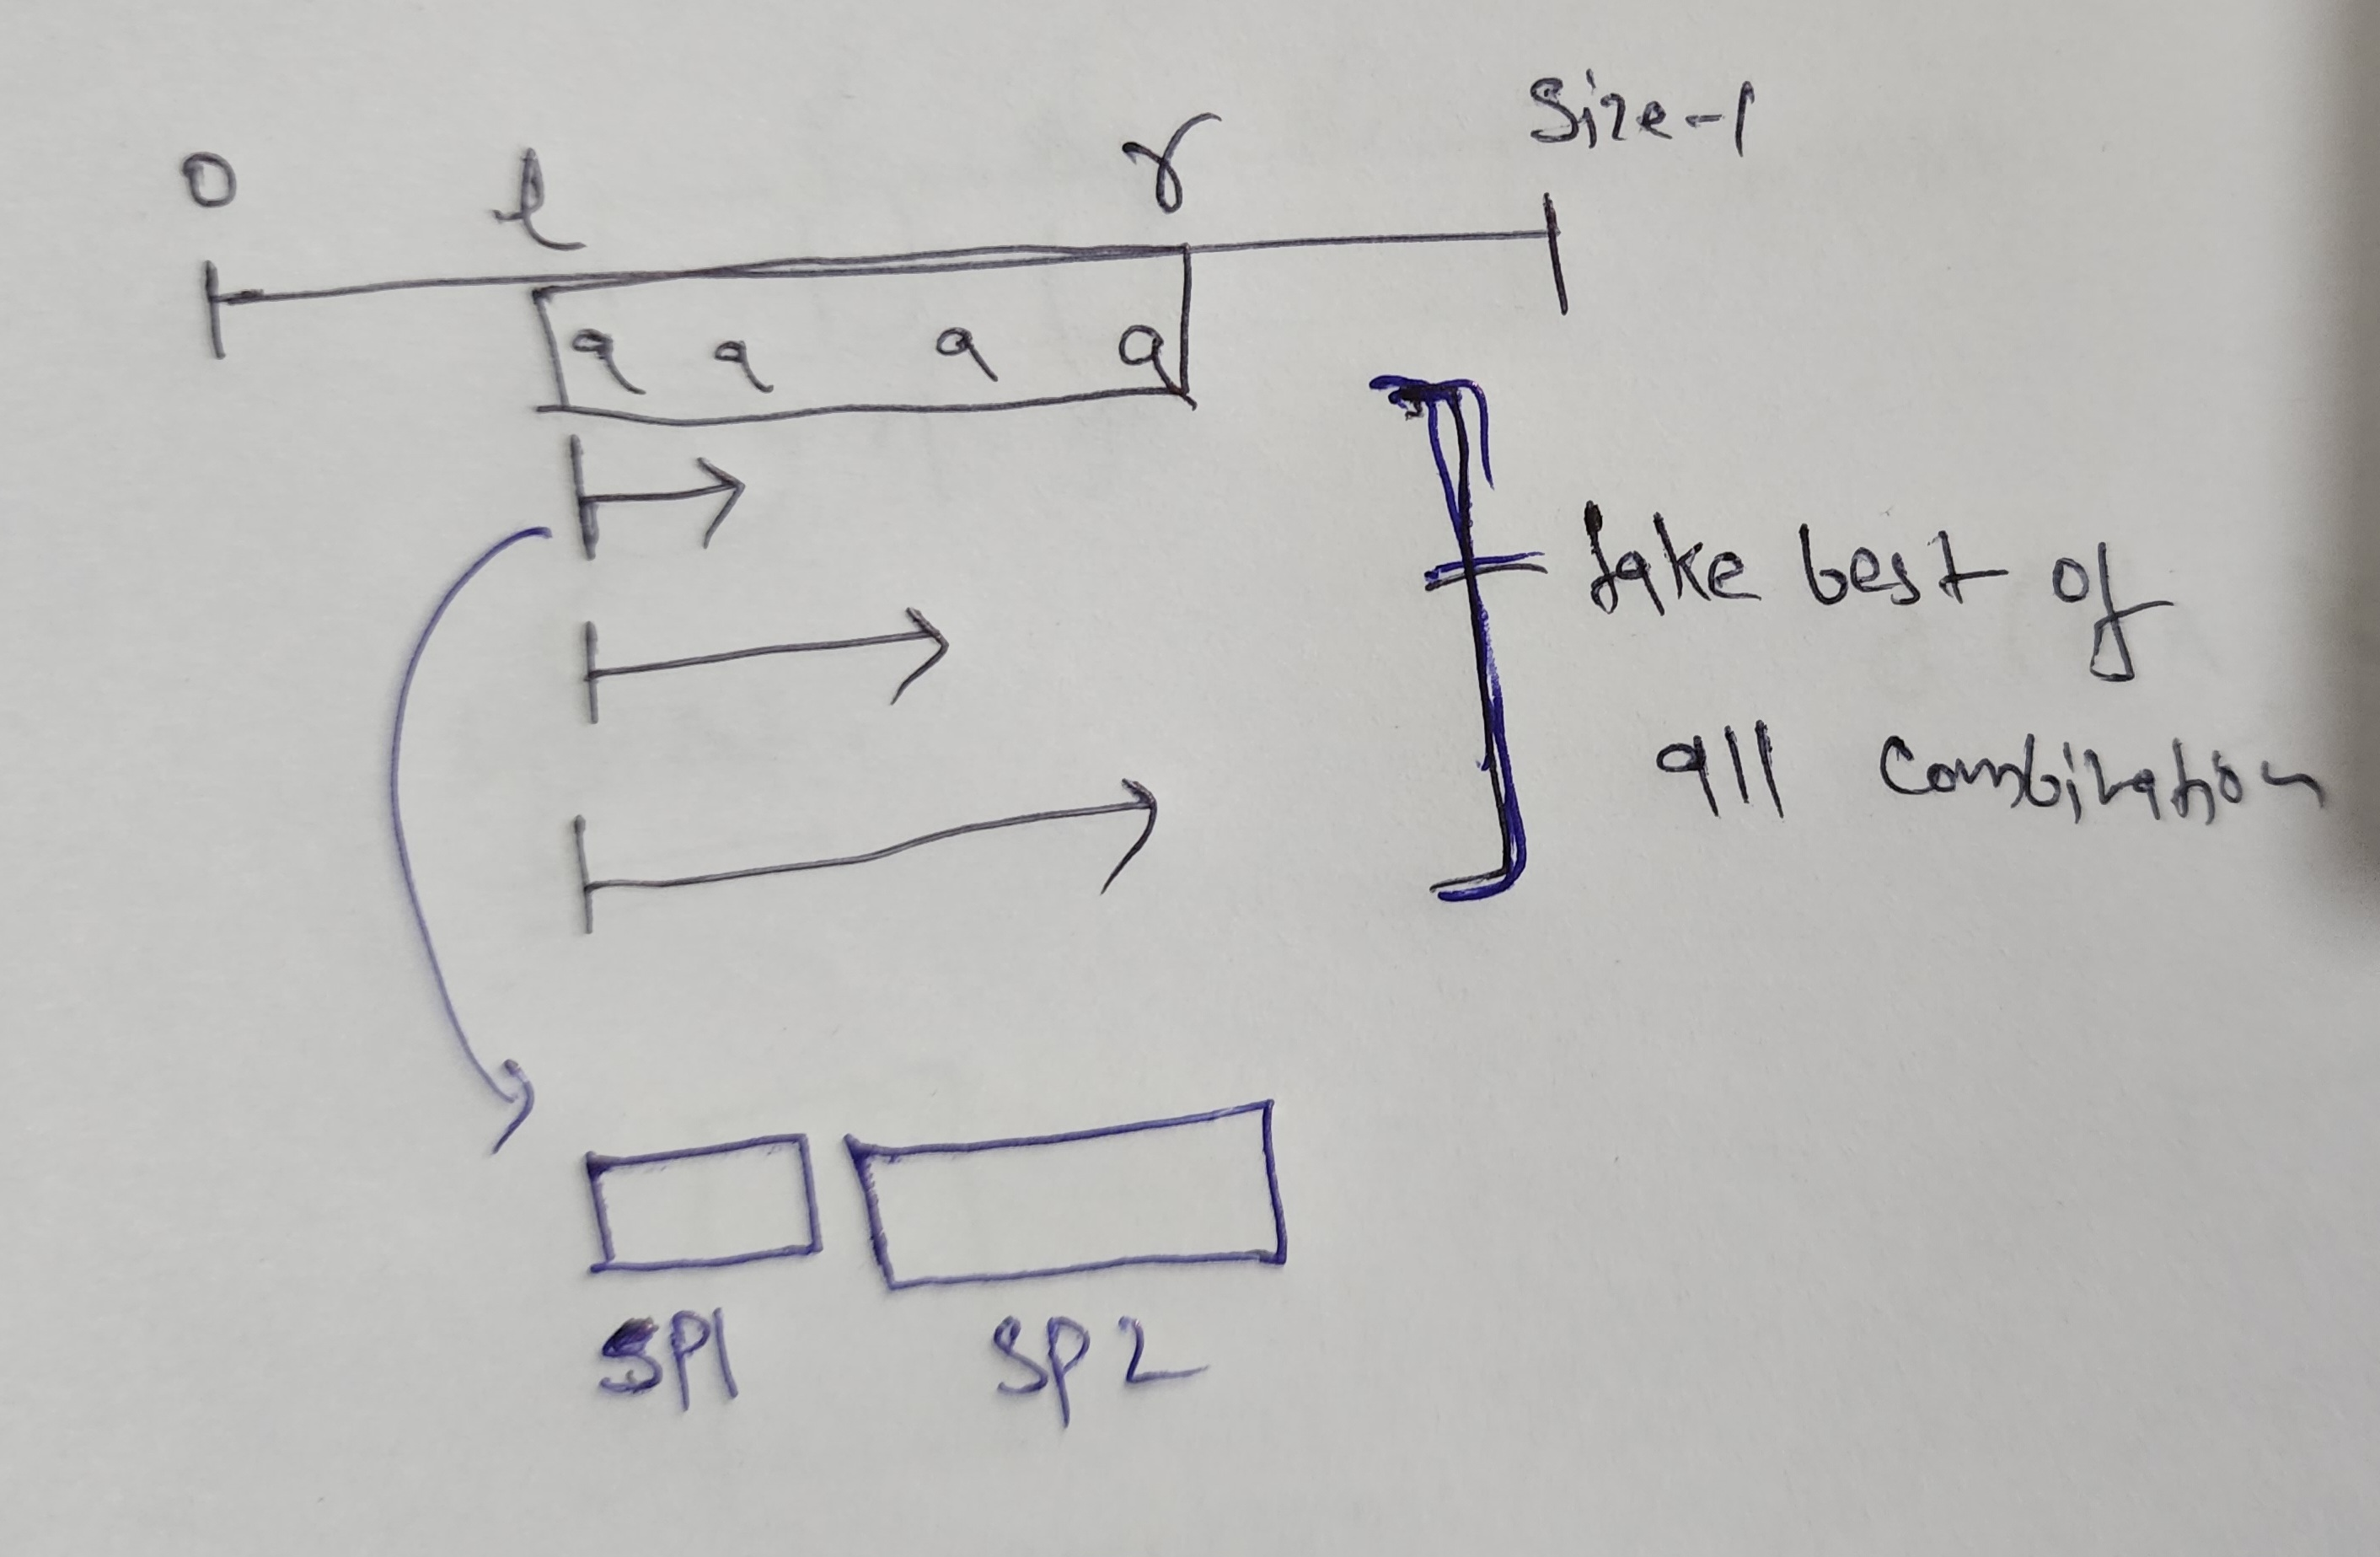
\includegraphics[width=\marginparwidth]{./resources/LC1246_p1.jpg}
    \end{enumerate}
    
\end{exerciseHints}